% !TeX document-id = {b3248781-f0ec-4e3d-85e3-e63d337a63f8}
% !TEX TS-program = tex
\documentclass[a4paper, 12pt]{article}

\usepackage{a4wide}
\usepackage[utf8]{inputenc}
\usepackage[russian]{babel}
\usepackage[pdftex]{graphicx}
\usepackage{amsmath}
\usepackage{amssymb}
\usepackage{amsfonts}
\usepackage{graphicx}
\usepackage{hyperref}
\usepackage{verbatim}
\usepackage{indentfirst}
\usepackage{listings}
% \usepackage{minted}
\setlength{\parindent}{1.25cm}

\newtheorem{myComment}{Замечание}
\newtheorem{myDef}{Определение}
\newtheorem{myProp}{Свойство}
\newtheorem{myTeor}{Теорема}
\newcommand{\dbtilde}[1]{\accentset{\approx}{#1}}
\newcommand{\cd}[1]{\lstinline$#1$}
\DeclareMathOperator{\sign}{sign}

\begin{document}
	
	\thispagestyle{empty}
	\lstset{language=C++}
	
	\begin{center}
		\vspace{-3cm}
		
\includegraphics[width=0.5\textwidth]{msu.png}\\
		{\scshape Московский государственный университет имени}\\
		М. В. Ломоносова\\
		Факультет вычислительной математики и кибернетики\\

		
		\vfill
		
		% {\LARGE Отчёт по практикуму}
		
		\vspace{1cm}
		
		% {\Huge\bfseries <<Оптимальное управление>>}\\
		{\LARGE Описание языка программирования Frigate}
	\end{center}
	
	\vspace{1cm}
	
	\begin{flushright}
		\large
		\textit{Студент 415 группы}\\
		А.\,Н.~Ашабоков
		
		\vspace{5mm}
		
		\textit{Руководитель практикума}\\
		к.ф.-м.н., А.Н. Сальников 
	\end{flushright}
	
	\vfill
	
	\begin{center}
		Москва, 2019
	\end{center}
	
	\newpage
	\setcounter{tocdepth}{1}
	\tableofcontents
	
	\newpage
	\normalsize
	
	\section{Общие сведения}
	
	Система Frigate позволяет программисту представить свой алгоритм в виде графа состоящего из множества непересекающихся по вершинам подграфов. Каждый подграф является графом в смысле системы PARUS. Подграфы поочередно назначаются на исполнение. Этим управляет процесс координатор, адрес которого знают все вершины. Координатор содержит условные выражения, соответствующие каждому подграфу. На исполнение назначается тот подграф, чье выражение истинно. Данный механизм позволяет динамически перестраивать граф-программу во время выполнения, назначая на выполнение один из заранее подготовленных подграфов в каждый момент времени.
	Ребра в графе бывают трех типов: внутренние (на уровне одного подграфа), внешние (на уровне графа соединяют подграфы), управляющие (на уровне графа направлены к процессу координатору). В целях уменьшения дублирования кода при создании большого количества подобных вершин или ребер был введен механизм шаблонов. Суть его в том, что программистом описывается шаблон вершины или ребра, содержащий все внутреннее устройство элемента, а при создании однотипных вершин или ребер, они используют описанный шаблон.
	Вершины в графе Frigate могут иметь несколько точек входа и выхода ребер, чередующиеся с блоками обработки кода, таким образом достигается более сложная логика в работе кода вершины.
	Программист описывает программу в синтаксисе языка Frigate, выделяя в программе последовательные участки обработки, соответствующие вершинам графа, и зависимости по данным - ребра. По данному представлению генерируется набор объектов в памяти, соответствующей иерархии классов. Затем из объектов-контейнеров генерируется набор функций с MPI- вставками, который компилируется на распределенной системе и связывается с подсистемой запуска.
	
	\begin{center}
		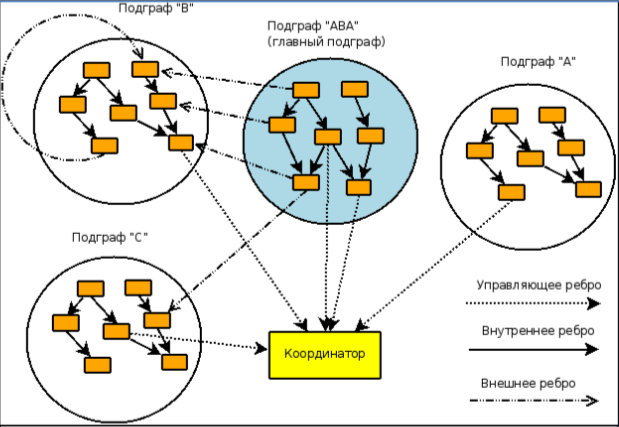
\includegraphics[width=0.7\textwidth]{pic_1.png}\\
		Рис. 1: Общая схема графа программы на языке Frigate. \label{pic_3}
	\end{center}
	
%	Программа на языке Frigate имеет следующую структуру:
%	
%	\begin{lstlisting}
%	<graph>
%	# Version of language
%	version = 1.0
%	
%	<header>
%	# the block that is copied to the beginning of the program
%	@
%	# block with C++ code
%	@
%	</header>
%	
%	<root>
%	# block that runs at the 
%	# very beginning of program execution
%	root="file_with_root_code"
%	</root>
%	
%	<tail>
%	# block that runs at the end of program execution 
%	</tail>
%	
%	<parameters>
%	# block containing a description of the parameters
%	var i = ("param_value_1" "param_value_n")
%	var j = ("param_value_1" "param_value_m")
%	...
%	</parameters>
%	
%	# name of main subgraph
%	main_subgraph="main"
%	
%	<subgraph>
%	# subgraph description 
%	name = "name_of_subgraph"
%	condition = @ fulfillment condition @
%	
%	<vertex>
%	# description of a vertex using a template
%	name = "name_of_vertex"
%	template = "name_of_vertex_template"
%	</vertex>
%	
%	<vertex>
%	# vertex description
%	name = "name_of_vertex"
%	
%	<code>
%	@
%	# some code 
%	@
%	</code>
%	
%	<exchange>
%	name = "name_of_exchange_block"
%	send = "name_of_edge"
%	...
%	recv = "name_of_edge"
%	</exchange>
%	...
%	<exchange>
%	...
%	</exchange>
%	
%	<code>
%	...
%	</code>
%	</vertex>
%	
%	<internal_edge>
%	# internal edge description
%	name = "name_of_internal_edge"
%	template = "name_of_template"
%	send = ("name_of_sender_vertex", 
%	"name_of_sender_exchange_block")
%	recv = ("name_of_receiver_vertex", 
%	"name_of_receiver_exchange_block")
%	</internal_edge>
%	
%	...
%	
%	<control_edge>
%	# control edge description 
%	name = "name_of_control_edge"
%	template = "name_of_control_edge"
%	send = ("name_of_sender_vertex", 
%	"name_of_sender_exchange_block")
%	</control_edge>
%	</subgraph>	
%	
%	...	
%	
%	<subgraph>
%	...
%	</subgraph>
%	
%	<external_edge>
%	# external edge description 
%	name = "name_of_external_edge"
%	template = "name_of_edge_template"
%	send = ("name_of_sender_subgraph", 
%	"name_of_sender_vertex", 
%	"name_of_sender_exchange_block")
%	recv = ("name_of_receiver_subgraph", 
%	"name_of_receiver_vertex", 
%	"name_of_receiver_exchange_block")
%	</external_edge>
%	
%	...
%	
%	<edge_template>
%	# edge template description 
%	name = "name_of_edge_template"
%	
%	<send>
%	# msg description
%	<fragment>
%	# data description
%	variable = @   @
%	type = @   @
%	left = @   @
%	right = @   @
%	</fragment>
%	...
%	<fragment>
%	...
%	</fragment>
%	</send>
%	
%	<recv>
%	...
%	</recv>
%	</edge_template>
%	...
%	
%	<vertex_template>
%	# vertex template description 
%	name = "name_of_vertex_template"
%	
%	<code>
%	io_volume = @ ... @
%	file = "name_of_file_with_code"
%	</code>
%	...
%	<code>
%	io_volume = @ ... @
%	code_volume = @ ... @
%	@
%	# code block
%	@
%	</code>
%	...
%	<exchange>
%	name = "name_of_exchange_block"
%	send = "name_of_edge"
%	..
%	recv = "name_of_edge"
%	</exchange>
%	</vertex_template>
%	</graph>
%	\end{lstlisting}

	\section{Структура языка}
	Данный раздел содержит описание структуры языка \cd{Frigate}. Для наглядности \hyperref[sec_3]{раздел 3} содержит пример кода.\\
	Перед началом разбора структуры языка введем следующие договоренности:
	\begin{itemize}
		\item Поле \lstinline$name$ внутри любого из объектов содержит имя данного объекта
		\item Блок вида $@$...$@$ содержит некоторый исполняемый код на языке C++. Пример:
		\begin{lstlisting}
		@
		int a = 1;
		int b = 2;
		int c = a + b;
		@
		\end{lstlisting}
	\end{itemize}
	Программа на языке Frigate описывается в виде графа, внутри блока <graph> содержится описание всех подграфов \lstinline$<subgraph>$, шаблонов вершин \lstinline$<vertex_template>$, шаблонов ребер \lstinline$<edge_template>$ и внешних ребер \lstinline$<external_edge>$, соединяющих вершины различных подграфов, а также содержит блоки \lstinline$<header>$, \lstinline$<root>$, \lstinline$<tail>$ и \cd{<parameters>}. 
	\begin{itemize}
		\item Блок \lstinline$<header>$  содержит в себе код на языке \lstinline$C++$, который при компиляции MPI программы будет прямиком скопирован в его начало. 
		\item Блок \lstinline$<root>$ содержит код C++, который выполняется MPI программой перед началом каких-либо действий. Его имеет смысл использовать для проведения подготовительных работ перед началом работы основного вычислительного алгоритма, например для инициализации каких-либо глобальных переменных и выделения памяти. 
		\item Блок \lstinline$<tail>$ содержит код \lstinline$C++$, который выполняется каждой вершиной по завершению основных вычислений. Данный блок можно использовать, например, для очищения выделенной памяти. 
		\item Блок \cd{<parameters>} содержит перечисление переменных-параметров и списки значений параметров для каждого из них. Параметры в языке нужны для имитиции работы цикла, а именно, для создания большого числа однотипных вершин, ребер и других сущностей, отличающихся только значением параметра. Например, при выполнении следующего кода будут созданы внутренние ребра c именами \cd{int\_1} и \cd{int\_2}, отличающиеся только значением в поле \cd{recv}: \cd{\"sub\_1\_vert\_2\"} и \cd{\"sub\_1\_vert\_3\"} соответственно.
		\begin{lstlisting}
			...
			<parameters>
			var i = ("1" "2")
			var j = ("2" "3")
			</parameters>
			...
			<internal_edge>
			using i, j;
			name = "int_%i%"
			template = "edge_template"
			send= ("sub_1_vert_1", "ex_1")
			recv = ("sub_1_vert_%j%", "ex_1")
			</internal_edge>
		\end{lstlisting}
		Поле \cd{using} содержит перечисление параметров, использующихся в данной сущности. Это поле является необязательным, т.е. если в описываемом объекте нет необходимости использовать параметры, поле \cd{using} можно не писать. Далее при описании полей ребер, вершин и других объектов, описание поля \cd{using} будем опускать.
		\item Поле \lstinline$main_subgraph$ содержит имя подграфа, который далее будет считаться главным.
	\end{itemize}
	Рассмотрим теперь структуру подграфа \lstinline$<subgraph>$. Подграф содержит описание все своих вершин \lstinline$<vertex>$, внутренних ребер \lstinline$<internal_edge>$ и управляющих ребер \lstinline$<control_edge>$. Сразу отметим, что эти блоки могут идти в произвольном порядке.
	\begin{itemize}
		\item Поле \lstinline$condition$ содержит условие выполнения данного подграфа на языке C++.
		\item Блок \lstinline$<vertex>$ содержит описание вершины данного подграфа. Вершины могут быть описаны либо явно внутри подграфа, либо при помощи шаблона вершины (см. далее), путем задания в поле \lstinline$template$ имя используемого шаблона. Очевидно, что использование шаблонов вершины имеет смысл в том случае, когда требуется создать большое количество однотипных вершин, реализующих один и тот же алгоритм. Явное описание вершины совпадает с описанием шаблона вершины и приведено далее по тексту. 
		\item Блок \lstinline$<internal_edge>$ содержит описание внутренних ребер подграфа. Очевидно, эти ребра могут быть использованы только для связи вершин внутри одного подграфа, для коммуникации с вершинами других подграфов необходимо использовать внешние ребра \lstinline$<external_edge>$. Внутреннее ребро содержит следующие поля:
		\begin{itemize}
			\item Поле \lstinline$template$ содержит название шаблона ребра, используемого данным ребром.
			\item Поле \lstinline$send$ содержит адрес отправителя в формате: $("$название вершины отправителя$"$, $"$название exchange блока отправителя$")$.
			\item Поле \lstinline$recv$ аналогично содержит адрес отправителя: $("$название вершины получателя$"$, $"$название exchange блока получателя$")$.
		\end{itemize}
		\item Блок \lstinline$<control_edge>$ содержит описание ребра, соединяющего вершину с координатором. Очевидно, что в \lstinline$<control_edge>$ нет необходимости описания адреса получателя. т.к. это всегда процесс-координатор. Структура ребра:
		\begin{itemize}
			\item \lstinline$template$ --- название используемого шаблона вершины.
			\item \lstinline$send$ --- адрес отправителя, в том же формате, что и для \lstinline$<internal_edge>$.
		\end{itemize}
	\end{itemize}
	Рассмотрим структуру блока \lstinline$<external_edge>$. Данный блок содержит описание внешней вершины, соединяющей вершины различных подграфов. Фактически структура внешнего ребра \lstinline$<external_edge>$ отличается от структуры внутреннего ребра \lstinline$<internal_edge>$ только набором параметром, задающих адрес отправителя и получателя. Это связано с тем, что при передаче данныз внутри определенного прдграфа, знание имени подграфа не является необходимым, что, очевидно, неверно для внешних ребер,
	\begin{itemize}
		\item Поле \lstinline$template$ содержит название используемого шаблона ребра.
		\item Поле \lstinline$send$ содержит адрес отправителя в формате: $("$название подграфа отправителя$"$, $"$название вершины отправителя$"$, $"$название exchange блока отправителя$")$.
		\item Поле \lstinline$recv$ аналогично содержит адрес отправителя: $("$название подграфа получателя$"$, $"$название вершины получателя$"$, $"$название exchange блока получателя$")$.
	\end{itemize}
	Рассмотрим структуру блока \lstinline$<edge_template>$. Этот блок содержит описание блоков памяти, содержащих данные для отправки по указанному ребру, и блоки памяти, в которые получаемые данные должны быть сохранены.
	\begin{itemize}
		\item Блок \lstinline$<send>$ содержит в себе перечисление некоторого числа блоков \lstinline$<fragment>$ ---  фрагментов памяти, подлежащих отправке по данному ребру. Блок \lstinline$<fragment>$ имеет структуру:
		\begin{itemize}
			\item Поле \lstinline$variable$ --- название переменной.
			\item Поле \lstinline$type$ --- тип передаваемых данных.
			\item Поле \lstinline$left$ ---  указатель на левую границу массива с данными в памяти.
			\item Поле \lstinline$right$ ---  указатель на правую границу массива с данными в памяти.
		\end{itemize}
		\item Блок \lstinline$recv$ содержит перечисление блоков \lstinline$<fragment>$ --- фрагментов памяти, в которые произойдет сохранение полученных по данному ребру данных. Структура блока \lstinline$<fragment>$ описана выше.
	\end{itemize}
	Рассмотрим структуру блока \lstinline$<vertex_template>$. Структура данного блока совпадает со структурой блока \lstinline$<vertex>$ в том случае, когда вершина задается не через шаблон вершины, а явно внутри блока \lstinline$<vertex>$. Блок \lstinline$<vertex_template>$ состоит из произвольного количества блоков \lstinline$<code>$ и \lstinline$<exchange>$ в произвольном порядке.
	\begin{itemize}
		\item Блок \lstinline$<code>$ содержит исполняемый код на языке C++. Его можно задать вписав код в специальный блок вида $@$...$@$, либо подключив файл с кодом на C++, указав название файла в поле \lstinline$file$.
		\item Блок \lstinline$<exchange>$ отвечает за обмен данными между вершинами. Управление обменом осуществляется при помощи полей \lstinline$send$ и \lstinline$recv$:
		\begin{itemize}
			\item Поле \lstinline$send$ содержит название ребра, по которому будет осуществляться отправка данных.
			\item Поле \lstinline$recv$ содержит название ребра, по которому будет осуществляться получение данных.
		\end{itemize}
		Дополнительно отметим, что блок \lstinline$<exchange>$ может состоять из произвольного количества полей \lstinline$send$ и \lstinline$recv$, перечисленных в произвольном порядке. Это значит, что один \lstinline$<exchange>$ блок может осуществлять произвольное число операций передачи и получения данных в произвольном порядке. Также стоит отметить, что возможно чередование блоков \lstinline$<code>$ и \lstinline$<exchange>$. Это значит, что вершина по мере выполнения может отправлять промежуточные данные и получать их от других вершин.
	\end{itemize}
	
	%\section{Соглашения об уникальности имен}
	%
	%Очевидно, что представление программы в виде графа может привести к тому, что полученный граф будет иметь довольно сложную структуру, что естественным путем приводит к необходимости введения пространств видимости имен.
	%
	%\begin{itemize}
	%	\item Имена подграфов \lstinline$<subgraph>$ не могут совпадать
	%	\item Имена вершин \lstinline$<vertex>$ внутри одного подграфа не могут совпадать
	%	
	%\end{itemize}
	
	\section{Пример кода}\label{sec_3}
	
	\begin{lstlisting}
	# test_3 
	# Answer: OK
	
	<graph>
	
	version = 1.0
	
	<header>
	@
	some code here
	@
	</header>
	
	<root>
	root = "root"
	</root>
	
	<tail>
	@
	some code here
	@
	</tail>
	
	<parameters>
	var i = ("1" "2")
	var j = ("2" "3")
	</parameters>
	
	main_subgraph = "sub_1"
	
	<subgraph>
	name = "sub_1"
	
	condition = @ some code here @
	
	<vertex>
	name = "sub_1_vert_1"
	
	<code>
	@
	some code here
	@
	</code>
	
	<exchange>	
	name = "ex_1"
	send = "int_1"
	send = "int_2"
	</exchange>
	</vertex>
	
	<vertex>
	name = "sub_1_vert_2"
	<code>
	@
	smdks
	@
	</code>
	
	<exchange>
	name = "ex_1"
	recv = "int_1"
	send = "ext_1"
	</exchange>
	</vertex>
	
	<vertex>
	name = "sub_1_vert_3"
	
	<code>
	@
	dwd
	@
	</code>
	
	<exchange>
	name = "ex_1"
	recv = "int_2"
	send = "cont_1"
	</exchange>
	</vertex>
	
	<control_edge>
	name = "cont_1"
	template = "edge_template_1"
	send = ("sub_1_vert_3", "ex_1")	
	</control_edge>
	
	<internal_edge>
	using i, j;
	name = "int_%i%"
	template = "edge_template"
	send= ("sub_1_vert_1", "ex_1")
	recv = ("sub_1_vert_%j%", "ex_1")
	</internal_edge>
	
	</subgraph>
	
	<subgraph>
	name = "sub_2"
	condition = @ some code here @
	
	<vertex>
	name = "sub_2_vert_1"
	
	<code>
	@
	kd
	@
	</code>
	
	<exchange>
	name = "ex_1"
	send = "int_1"
	send = "int_2"
	</exchange>
	
	</vertex>
	
	<vertex>
	name = "sub_2_vert_2"
	
	<code>
	@
	sfe
	@
	</code>
	
	<exchange>
	name = "ex_1"
	recv = "int_1"
	recv = "ext_1"
	</exchange>
	</vertex>
	
	<vertex>
	name = "sub_2_vert_3"
	
	<code>
	@
	jnfkn
	@
	</code>
	
	<exchange>
	name = "ex_1"
	recv = "int_2"
	</exchange>
	</vertex>
	
	<internal_edge>
	using i, j;
	name = "int_%i%"
	template = "edge_template"
	send= ("sub_2_vert_1", "ex_1")
	recv = ("sub_2_vert_%j%", "ex_1")
	</internal_edge>
	
	
	</subgraph>
	
	<edge_template>
	name="edge_template"
	<send>   
	<fragment>
	variable = @ some code here @
	type     = @ some code here @
	left     = @ some code here @
	right    = @ some code here @
	</fragment>
	</send>
	
	<recv>
	<fragment>
	variable = @ some code here @
	type     = @ some code here @
	left     = @ some code here @
	right    = @ some code here @
	</fragment>
	</recv>
	</edge_template>
	
	<external_edge>
	name = "ext_1"
	template = "edge_template"
	send = ("sub_1", "sub_1_vert_2", "ex_1")
	recv = ("sub_2", "sub_2_vert_2", "ex_1")
	</external_edge>
	</graph>
	
	
	\end{lstlisting}
	
	\section{Структура проекта}
	
	Проект имеет следующую структуру:
	
	\begin{itemize}
		\item \cd{Parser/}
		\begin{itemize}			
			\item \cd{Tag.h} содержит классы, соответствующте всем лексемам грамматики, напрмер: \cd{StringTag} --- обозначает набор символов вида: "some\_string".
			
			\item \cd{LexTag.h} содержит производные тэги, полученные из базовых лексем, напрмер: \cd{main_subgraph} --- производный тэг, состоящий из лексем \cd{MainSubgraphTag}, \cd{AssignTag} и \cd{StringTag}, ему соответствует фрагмент программы: \\
			\cd{main_subgraph = "name_of_main_subgraph"}.
			
			\item \cd{Lexer.h} содержит класс \cd{Lexer} с полями \cd{text} и \cd{tagMap}, и функцией \cd{go}. Конструктор класс получает на вход строку, содержащую весь код программы на языке \cd{frigate} и записывает его в поле \cd{text}. Далее функция \cd{go} производит разбор текста на лексемы, описанные в \cd{Tag.h}.
			
			\item \cd{Parser.h} содержит класс \cd{Parser}, который производит рекурсивную свертку из списка лексем типа \cd{Tag} к единственному тэгу \cd{graph}. В случае неудачи, вызывается ошибка. Описание правил свертки для каждого тэга описано в соответствующем классе в файле \cd{LexTag.h}.
			
			\item \cd{HexParser.h}  содержит функцию \cd{parse} --- производит лексический и синтаксический разбор исходного текста, а также проверяет результат на правильность и вызывает исключения, если нужно.
		\end{itemize}
		\item \cd{Exteptions/}
		\begin{itemize}
			\item \cd{Exception.h} содержит класс исключений \cd{Exception} --- крайне простой класс с двумя полями: название исключения (для классификации ошибок) и сообщение.
		\end{itemize}
		\item \cd{Compiler/}
		\begin{itemize}
			\item \cd{ControlEdge.h} содержит класс, обозначающий управляющее ребро. Имеет следующие поля:
			\begin{itemize}
				\item \cd{name} --- название ребра (везде далее при описании других классов будем опускать описание этого поля, т.к. из названия поля очевидно его назначение).
				\item \cd{send_coord} --- адрес отправителя.
				\item \cd{sends} --- вектор фрагментов для отправки.
				\item \cd{recvs} --- вектор фрагментов для чтения.
			\end{itemize}
			Список методов:
			\begin{itemize}
				\item \cd{addSendFragment} и {addRecvFragment} --- сеттеры для полей \cd{sends} и \cd{recvs}.
				\item \cd{readTag} --- метод заполняет поля класс, извлекая информацию из тэгов (этот метод тоже часто встречается в других классах и используется также,  так что ниже будем опускать его описание).
				\item \cd{emplaceParams} --- в язык была добавлена возможность создания объектов (в том числе и ребер) с использованием параметров в названиях (см. выше описание возможностей языка). Эта функция занимается работой с этими параметрами.
			\end{itemize}
			\item \cd{Coords.h} содержит классы (названия классов соответствуют грамматике языка, а назначение --- описанию языка выше):
			\begin{itemize}
				\item \cd{Coord} --- класс, описывающий адрес для работы с ребрами.
				\item \cd{CodeBlock} --- класс, содержащий описание кода на языке Си.
				\item \cd{Fragment} --- класс, с данными, описывающими фрагмент памяти, с которым будет работать ребро при отправке и получении сообщений.
			\end{itemize}
			\item \cd{Exchange.h} содержит единственный класс \cd{Exchange}, который отвечает за описание блока обмена данными в теле вершины. Названия полей совпадают с названиями соответствующих элементов языка \cd{frigate}, смысл тоже.
			\item \cd{ExternalEdge.h} содержит одноименный класс, описывающий ребра, соединяющие вершины в разных подграфах. Поля и методы аналогично \cd{ControlEdge}, с тем лишь исключением, что в этом ребре появилось поле, содержащее как адрес отправителя, так и адрес получателя.
			\item \cd{internalEdge.h} содержит одноименный класс, описывающий ребра, соединяющие вершины в пределах одного подграфа. Описание полей аналогично \cd{ExternalEdge}.
			\item \cd{Vertex.h} содержит описание класс \cd{Vertex}, реализующего вершины. Поле \cd{template_name} содержит название шаблона вершины (если объект вершины создается с помощью шаблона вершины) или пустую строку (если шаблон вершины не используется). Поле \cd{body} содержит перечисление объектов типа \cd{Exchange} и \cd{CodeBlock}, т.е. задает тело вершины. Помимо описаных выше функций \cd{readTag} и \cd{emplaceParam}, класс содержит функции \cd{rebindSend} и \cd{rebindRecv}. Эти функции подставляют значения параметров в адресные поля \cd{Exchange}, т.е., к примеру, из \cd{\"vert\_\%i\%\"} делает  \cd{\"vert_1\"}.
			\item \cd{Subgraph.h} содержит класс, описывающий подграф. Поле \cd{condition} содержит условие выполнения подграфа. Поля \cd{verticies}, \cd{internal_edges} и \cd{control_edges} содержат соответственно перечисления вершин, внутренних и управляющих ребер подграфа. Помимо стандартного набора сеттеров, имеется функция \cd{cyclic}, которая отвечает за проверку на цикличность, т.е. проверяет подграф на наличие циклов и вызывыает соответствующее исключение, если цикл есть.
			\item \cd{Graph.h} содержит класс \cd{Graph}, который описывает структуру графа. Назначение полей \cd{version}, \cd{header}, \cd{root}, \cd{tail} и \cd{main_subgraph} очевидно из названия, они содержат информацию, хранящуюся в соответствующих блоках разбираемого кода. Поля \cd{subgraphs} и \cd{external_edges} содержат перечисления подграфов и внешних ребер, из которых состоит граф. Функция \cd{validate} подставляет значения параметров в названия вершин, ребер и т.д., и проверяет получившиеся имена объектов на уникальность. Функция \cd{cyclic} производит проверку графа на наличие циклов. Функция \cd{prettyPrint} выводит структуру графа в формате \cd{dot}. 
			\item \cd{StaticHelper.h} содержит статичный класс с вспомогательными полями и функциями: 
				\begin{itemize}
					\item \cd{location_prefix} --- хранит путь до рабочей директории.
					\item \cd{readFile} --- функция чтения данных из файла.
					\item \cd{parameters} --- содержит имена параметров и множества значений.
					\item \cd{registerParam} --- добавляет новые параметры в \cd{map} параметров, параллельно проверяя его на уникальность.
					\item \cd{replaceAll} --- функция производит замену всех подстрок в строке.
				\end{itemize}
			\item \cd{crossvector.h} содержит описание класса, который может хранить в себе объекты двух различных типов в определенном порядке (самодельный вектор с поддержкой хранения объектов двух различных типов в определенном порядке). 
		\end{itemize}
	\end{itemize}
	
\end{document}